\documentclass[a4paper]{article}

\usepackage{graphicx,url}
\usepackage[T1]{fontenc}
\usepackage[latin1]{inputenc}

\usepackage{listings}
\usepackage{tabularx} % para igualar colunas (com largura automatica)

\def\framework{\textit{framework}}
\def\Framework{\textit{Framework}}

\usepackage[margin=3cm]{geometry}

\title{Resource Management for Embedded Systems}

\author{
  Roger Kreutz Immich, Diego Luis Kreutz and Ant�nio Augusto Fr�hlich\\
  Laboratory for Software and Hardware Integration\\
  Federal University of Santa Catarina\\
  PO Box 476 -- 88049-900 -- Florian�polis, SC, Brazil\\
  \{roger,kreutz,guto\}@lisha.ufsc.br\\
%  {\texttt{http://www.lisha.ufsc.br/}}
} 


\begin{document}

\maketitle

\begin{abstract}

  Classical strategies for resource management in operating systems are
  often complex and innapropriate for embedded systems. Implementations
  for these strategies may use either virtual function tables or long
  conditional structures to provide transparent access to different
  resources. This overhead is unacceptable for embedded systems. The
  EPOS operating system provides flexible and transparent access to
  resources for applications without incurring in unnecessary overhead.
  Metaprogrammed structures are used to predict, according to
  application usage and in compile time, whether a resource must use a
  polimorphic representation or may be accessed through direct calls.
  This way, virtual function tables are only used in the system when
  strictly necessary, and thus saving resources. In this article, we
  show that this strategy is a viable alternative for resource
  management in embedded systems.\\

\textbf{Keywords:} Resource Management, Static Meta-programmming, Operating Systems

\end{abstract}


\section{Introduction}


One of the main functions of an operating system is to manage hardware
and software resources in a transparent and efficient way. General
purpose systems often have to manage a great amount and variety of
resources. Classical strategies of resource management in operating
systems are thus often complex and dependent of application domain.

In order to provide application programmers with a reusable resource
management application programming interface (API), for example, through
a file system interface, general purpose systems often make use of
conditional structures or virtual function tables in their
implementation. The system doesn't know \emph{a priori} what type of
resource it must manage, and must provide access to all possible
resources through a common interface. This causes the system to
aggregate code blocks that may never be executed, but nonetheless will
ocupy system memory, and occurs in runtime overhead.

In embedded systems, applications typically use less resources than in
general-purpose system. If, for example, an embedded application uses a
single type of resource, an \emph{application-tailored} operating system
could provide management to that single resource, without incurring in
runtime overhead or aggregating unnecessary code blocks. If an
application, however, uses \emph{n} resources, this operating system
should also be able to provide a metamorphical, uniform interface for
managing these \emph{n} resources.

EPOS (Embedded Parallel Operating System) is an \emph{application
  oriented} operating system that provides an adaptive, flexible and
transparent interface for resource management\cite{Frohlich:2001}. 
Through the use of static metaprogramming techniques, and based on 
application analisys, it is possible to predict in compile time 
whether resources may be managed through a \emph{direct call} or 
\emph{polimorphic} interface. This way, only the absolutelly 
necessary overhead is introduced into the system.

This paper elaborates on the resource management strategy in EPOS.
Section~2 presents the EPOS metaprogrammed resource management
framework. Section~3 evaluates the strategy, presenting a case study
and evaluating overhead and performance of resource management in EPOS.
%eCOS~\cite{ecos} and uCLinux~\cite{uclinux}. 
Section~4 discusses related work. Section~5 discusses the results and
finalizes.

%%%%%%%%%%%%%%%%%%%%%%%%%%%%%%%%%%%%%%%%%%%%%%%%%%%%%%%%%%%%%%%%%%%%%%%%%%%%%%%%%

\section{ Resource Management in EPOS }

Resource management is a key point in operating system performance and
usability. In the particular case of \emph{application-tailored}
operating systems \cite{Frohlich:2001}, resource management is a specially
interresting problem, as the application itself defines what resources
must be managed in a given system instance, for a given execution
environment. The application programmer must be provided with reusable
interfaces, and with transparent component selection mechanisms.

\begin{figure*}[htb]
\centering
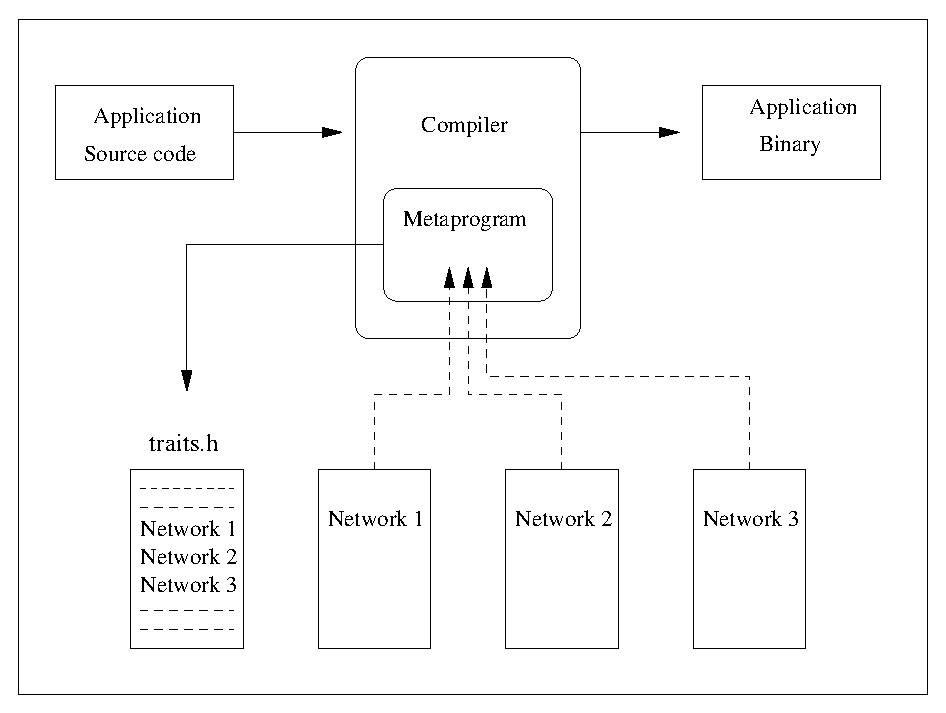
\includegraphics[width=.7\textwidth]{figuras/metaprograma-en.eps}
\caption{How the metaprogram works}
\label{metaprograma}
\end{figure*}

One way to deliver transparent, adaptative resource management in an
application oriented operating system is through the use of static
metaprogramming. Metaprogrammed frameworks allow the system to select
addequate components for resource management, generating flexible
interfaces that may either generate \emph{static} function calls or
\emph{virtual function tables}, according to application's needs and in
compile-time.

EPOS relies on a specially developed metaprogrammed library to provide
efficient and flexible resource management. Conditional structures (e.g.
\texttt{IF-THEN-ELSE} and operators \texttt{EQUAL} are defined by this
library, and implemented as described in \cite{robson:99:stl}. These library
functions are not restricted to resource management, and may be used
elsewhere in the system.

%%% n�o t� faltando uma explica��o espec�fica, ou um exemplo antes da figura?
%%% onde e como � usado, etc

Figure~\ref{metaprograma} illustrates the EPOS resource management
resolution process which is applied in compile time. In the first step,
macro components that satisfy user requirements are selected through
application code analisys \cite{fauze:2005}. In the second step, specific,
platform-dependent components are selected to become part of the
system's final instance. In this phase, the metaprogrammed framework
elliminates all virtual funcion call whenever possible, reducing final
object code size. 

As an example, if an application needs to use two network cards, the
programmer simply declares two NIC objects. In compile-time, the
application is analised according to the selected platform. The
metaprogrammed framework identifies the types of network cards available
in this instance of the system. If two network cards of different types
are available, the resource management interface for these cards will
present the same interface, and its implementation will be polimorphic.
If two network cards of the same type are available, the resource
management interface will still be uniform, but will provide direct
access to the actual device, with no virtual function call overhead.
This process requires no further user interaction than to select and
configure the target platform, and is transparent to the application.


\begin{figure}[tb]
\begin{center}
\begin{footnotesize}
\lstset{language=c++,frame=lrtb}
\lstset{basicstyle=\ttfamily}
\lstset{commentstyle=\textit}
\lstinputlisting{figuras/net.c}
\caption{Sample Application}
\label{aplicacaoexemplo}
\end{footnotesize}
\end{center}
\end{figure}

\begin{figure*}[tb]
\begin{center}
\begin{footnotesize}
\lstset{language=c++,frame=lrtb}
\lstset{basicstyle=\ttfamily}
\lstset{commentstyle=\textit}
\lstinputlisting{figuras/traits.c}
\caption{Description of the network cards in the traits file}
\label{traits}
\end{footnotesize}
\end{center}
\end{figure*}


Considering three hypothetical platforms "A", "B" and "C", and two
network cards "X" and "Y". The programmer might use a similar code to
the one presented in Figure~\ref{aplicacaoexemplo} for different all
three platforms. If that application were compiled for the hypothetical
platform "A", with two network cards of type "X", the polimorfism of
objects nic0 and nic1 will be replaced by direct calls to the actual
instances of the network cards "X". The same process would be repeated for a
supposed architecture "B", that has two network cards of type "Y". The
great advantage is that the user application continues the same one,
transparent and with a high degree of code reuse. On the other hand, the
polimorfism could not be eliminated for platform "C", because, it makes
use of one network card "X" and another network card "Y".  In this in case, it
is only possible to determine which calls goes to an specific network card
in runtime.


\subsection{ Resource Management Metafunctions}

A metaprogrammed \texttt{LIST} construct is used to generate a metalist
in compile-time wich contains the available resources of a given type in
the system. An configuration repository contains details regarding
configuration and characteristics of all resources that may be used in a
given platform. Figure~\ref{traits} illustrates a sample traits
configuration archive for the PC platform (Intel IA32 Architecture) in
EPOS. In that example, configuration values for number of sending and
receiving buffers are defined for three network devices:
\texttt{PCNET32}, \texttt{E100} and \texttt{C905}. This information will
be pertinent in compile time, during the definition of an instance of
the respective component.

The \texttt{polymorphic} construct returns a boolean value obtained
through the applicationa analisys in compile-time using the previously
defined metalist.  When the sistem is configured with different devices
of the same class (e.g. the PCNet32, E100 and C905 network cards defined
in figure~\ref{traits}), this construct returns \texttt{TRUE} indicating
that the use of the polimorfism will be necessary.  When the metalist
has only one element, or several elements with the same type, this
function returns \texttt{FALSE}, indicating that the polimorfism can be
eliminated and direct calls can be used to interact with the devices
present in the list.

The \texttt{polymorphic} construct is used in a metaprogrammed
conditional structure, that defines a \texttt{Base} variable (figure
\ref{polimorfismo}). The \textit{Base} will be either a pointer for
virtual methods (when polimorphic) or a pointer to an actual device
(when not polimorphic), allowing direct calls to the device. 

\begin{figure}[tb]
\begin{center}
\begin{footnotesize}
\lstset{language=c++,frame=lrtb}
\lstset{basicstyle=\ttfamily}
\lstset{commentstyle=\textit}
\lstinputlisting{figuras/metaif.c}
\caption{Conditional Structures for Removing Polimorphism}
\label{polimorfismo}
\end{footnotesize}
\end{center}
\end{figure}


\section{Evaluation}

In order to test the efficiency of resource management in the EPOS, a
simple application was implemented that sends the "A" caracter through
the network interfaces. Two sample target configurations were use: one
with a single network card, and another with two different types of
network cards. This experiments demonstrates the percentage of resource
management that is eliminated when virtual function calls are removed
from the system.

We developed and compiled this application for the IA-32 architecture.
Table \ref{tab-tamanho} presents data and code memory sizes for test case A
(concrete) and B (polimorphic). These values demonstrate that the
resources management in the EPOS carried through in compile time,
optimizes memory usage, allocating space only for the resources that
really will be used in the application in question.


\begin{table}[ht]
\begin{center}
\begin{tabular}{|c|c|c|}
\hline
	&Test Case A & Test Case B \\
\hline
.text	&19308		&19668	\\
\hline
.data	&88		&88	 \\
\hline
.bss	&432		&432      \\
\hline
\end{tabular}
\caption{Size in bytes for the Test Case A (Single NIC) and B (Two Different NICs) }
\label{tab-tamanho}
\end{center}
\end{table}

In a second experiment, we measured the access time to resources in the
EPOS system. The measurements were taken by measuring the time
immidiatly befre calling the \texttt{send} method, and when entering the
actual \texttt{send} method in the NIC driver. We executed 100 iterations with
1000000 measurements each over a VMWare emulator in an Athlon64 3000 machine.
Table~\ref{tab-tempo} presents access time in microseconds for both test cases.
These measurements
demonstrate the efficiency of removing polimorphism whenever possible in
a resource management strategy.

\begin{table}[tb]
\begin{center}
\begin{tabular}{|c|c|c|}
\hline
	&Test Case A & Test Case B \\
\hline
Time	& 13.6		& 14.61	\\
\hline
\end{tabular}
\caption{Time in microseconds for access to a NIC in Test Case A and B }
\label{tab-tempo}
\end{center}
\end{table}

Through the use of the resource management strategies in EPOS it is
possible to provide memory economy and to improve the access time to the
resources.  Memory economy is reached through the elimination of
everything that is not be to the application execution, leaving the
final code tailored to this application. The improvement in the access
time to the peripherals is reached replacing, in compile time, virtual
methods for direct calls.

\section{Related Work}

Boost \cite{Gurtovoy:2005:Boost} C++ is a library of metafunctions that
can be used for the most diverse intentions.  Boost intent to group
important abstractions of functional and generic programming to
construct a set of tools, in turn easy to use, capable to become the
metaprogramming through templates to practical sufficient for real
environments.  In its conception, the Boost library is strong influenced
by STL library (Standard Template Library ). While the first one is
decided in compile time second is decided in runtime, what it provides a
differential that will be able to make the difference in accordance with
the context. An application for an embedded system could demand the
resolution of the biggest part (or all) the dependences in compile time
(therefore systems embedded normally has limited resources, being
unprovided of special areas of storage - as hard disks - and possessing
reduced amounts of RAM memory).  On the other hand, an usual
application, destined the general purpose microcomputers, can have no
restriction to how much use of libraries (metafunctions, class,
algorithms, etc) that they will be resolved/loaded in runtime.


The aspcect mining \cite{Deursen:2003:Aspect, griswold00aspectbrowser,
  Breu:2004:Aspect, Deursen:2005:A, Hannemann:2005:aosd05} is a research
line that has for objective the analysis and development of tools that
allow the identification of aspects that can be refactored, based in
object-oriented programming languages. The basic idea is the search for
aspects spread for the code, trying groups them by similarity in
intention to separate the common parts, providing the refactoration of
the software.

Despite the some research in the area of aspect mining and refectoring
still has no solutions or tools capable to identify and to isolate all
the possible aspects for refactoring in a software.  This is a
sufficiently complex task, that demands one high degree of knowledge
concerning the programming languages and its capacities of
representation and organization of data and algorithms.  To complement
to this still exists the complication of the different forms that a
programmer can implement and represent a solution for the problem.
These factors increase the identification difficulty and aspects
refactoring, that becomes still more complicated in flexible and rich
programming languages.

The object-oriented programming languages bring mechanisms that
facilitate code reuse. Between them can be cited the polimorfism,
inheritance, metaprogramming, encapsulation and dynamic linking. All
these resources looking for to facilitate the life of the programmers
and/or to provide flexibility in levels before unattachable. In the
context of embedded systems two of these mechanisms are at the same time
desirable, however impracticable, the polimorfism and the dynamic
linking. These mechanisms supply attractive ways to resolution of
different computational problems, however, they bring overheads (of
memory and processing) what is not acceptable in the majority of the
embedded systems. An ideal situation would be where the developer could
make use of these resources in codification time and the same ones were
eliminated in compile time, preventing the extra consumption of
resources in runtime.

In current literature exist some proposals of refatoring, browsers and
aspect mining.  However they are in phase of development and/or
experimentation and still is not possible to evidence, with the result
gotten until the moment, if these could be applied in embedded systems.
The aspect refactoring was considered by
Hanenberg\cite{hanenberg03refactoring} and has as objective to
reorganize the aspects, favoring the flexibility and the legibility of
the code.  However it does not eliminate the polimorfism, and of this
form, it is not adjusted for embedded systems.

The proposal of use aspect browsers with the objective of assisting in
the recognition of standards and facilitating the navigation between
them, also already was explored
\cite{griswold00aspectbrowser,janzem03navigating}. However it requires
that the developer have a great knowledge of the guided paradigm of
aspect programming, as of the tool that will be used and equally the
refactoring, it not to provide the identification with points where the
polimorfism can be substituted by direct calls.
 
Aspect Mining \cite{tourwe04codemining} uses the technique of formal
concept analysis\cite{wille81restructuring} to find automatically
stretches of code with transversal functionalities to the system in
methods, class and hierarchy of class, that are correlated of some way.
This approach is in initial phase of experimentation and still does not
present expressive resulted for the case of polimorfism.

The basic objective of the virtual functions (as the \texttt{virtual} in
C++) is to facilitate code reuses\cite{Bacon:1996:Fast,
  Driesen:1996:The}. However, this function can produce a great increase
of complexity.  In this direction, some initiatives come being done in
the search for solutions that they aim at to reduce, in a transparent
form, the impact in the performance and size of the code when use
virtual functions.  The objective of research as \cite{Bacon:1996:Fast}
and \cite{Driesen:1996:The} is to provide tools for the analysis and
reduction the unnecessary code.  Some results show that it is possible
to decide up to 71\% of the virtual functions and to reduce the compiled
code in 25\%.  Also it was demonstrated that some algorithms are
sufficiently fast and could be good chances for the inclusion in C++
compilers.


\section{Conclusion}

The use of the static metapramming techniques to provide optimization in
the resources management strategies for EPOS revealed a viable
alternative for embedded systems.  Despite the difficulties introduced
by metaprogramming constructs, such as the increase of the complexity,
difficulty of depuration and greater compile time, it was shown that
that it is possible to use isolate its usage in the system only in the
places where it becomes necessary, keeping the original structure in the
others parts, continuing with the original flexibility and providing the
necessary optimization. Current work focuses on further evaluating this
techniques, and comparing it to other existing solutions.







\bibliographystyle{plain}
\bibliography{metatool}

\end{document}
